The field of protein engineering has witnessed many advancements in recent years, fueled by the growing demand for designing novel proteins with enhanced functionalities. In this context, machine learning techniques have emerged as powerful tools for analysing and manipulating proteins. 

Many state-of-the-art approaches that use machine learning focus on the sequence of a protein, rather than its structure, because protein sequences are more widely available. In this chapter, we explore the existing body of literature surrounding the most powerful techniques to assess the fitness of mutations, as well as discussing the emerging techniques that aim to take advantage of the structure of proteins by highlighting the key contributions, methodologies, and findings that have paved the way for this research area.

\section{Sequence-based protein engineering}

\subsection{Multiple sequence alignments}
Many approaches to protein engineering use multiple sequence alignments (MSAs) to study and propose mutations for each protein sequence. In bioinformatics, sequence alignment refers to arranging sequences of proteins to identify regions of similarity that may indicate evolutionary relationships, which provide insight into the function of the aligned proteins. By training machine learning models on MSAs, a coordinate system of the aligned sequences is developed, allowing the model to score amino acids at a given position and to compare them to the rest of the training set. This was the approach taken first by \citet{deepsequence}, who propose a Variational Autoencoder, DeepSequence, trained on protein-specific MSAs to understand the most likely amino acids to be present at certain positions in the sequence. This approach was later expanded by \citet{EVE}, who proposed EVE, a model that predicts the fitness of human variants in disease-related genes. 

\subsection{Large language models}
% The usage of MSAs, however, has some limitations. Most importantly, they cannot deal with non-alignable proteins; these are proteins have diverged significantly over evolutionary time and share very little sequence similarity with other proteins. In such cases, traditional sequence alignment methods may not be able to identify regions of similarity that help the models assess the quality of mutations. Due to this limitation, some researchers have started pursuing an alternative line of inquiry, in which models do not need MSAs.  This line of inquiry has taken advantage of the advances made in the Natural Language Processing field to understand sequences, with \citet{alley2019unified} and \citet{heinzinger2019modeling} each training Long Short-Term Memory Networks \cite{lstms} across many protein families.

% The rise of the Transformer architecture, first introduced by \citet{vaswani2017attention}, has resulted in significant performance improvements on sequence-based tasks. \citet{madani2020progen, nambiar2020transforming, rives2021biological} were the first to propose the usage of transformers to model protein sequences. In a line of research that combines both the usage of MSAs and the usage of large language models, \citet{Rao2020} introduced the MSA Transfomer, a model trained on a large collection of MSA families. In opposition, \citet{elnaggar2021prottrans} and \citet{meier2021language} developed transformers trained exclusively on non-aligned proteins from protein databases. In parallel, \citet{vig2020bertology} showed how the self-attention mechanism that is characteristic of the Transformer architecture actually captures the underlying structure of protein sequences and can build complex biophysical properties as the number of self-attention layers increases. 

While MSAs provide good evolutionary insights, they need to be re-trained for each protein of interest, and have difficulties dealing with non-alignable proteins that have diverged significantly over time. To address this, researchers have explored an alternative approach that leverages Natural Language Processing techniques. \citet{alley2019unified} and \citet{heinzinger2019modeling} trained Long Short-Term Memory Networks (LSTMs) to understand protein sequences across various families.

The Transformer architecture, introduced by \citet{vaswani2017attention}, has shown significant performance improvements for sequence-based tasks. \citet{madani2020progen, nambiar2020transforming, rives2021biological} proposed the use of transformers for modeling protein sequences. \citet{Rao2020} introduced the MSA Transformer, which combines MSAs and large language models. Conversely, \citet{elnaggar2021prottrans} and \citet{meier2021language} developed transformers exclusively trained on non-aligned proteins. Additionally, \citet{vig2020bertology} demonstrated how the self-attention mechanism in Transformers captures features that correlate with the structure of protein sequences and can model complex biophysical properties with increased self-attention layers.

Most recently, \citet{tranception} have proposed an auto-regressive transformer model, Tranception, that achieves state-of-the-art results on their newly compiled benchmark dataset, ProteinGym, that spans 87 DMS assays,\footnote{Deep mutational scanning is a high-throughput functional assay that measures the effect of every genetic change at every site in a protein.} containing the protein fitness of over 1.5M variants. However, as it will be shown in this project, while its performance ranks highest for predicting fitness across all variants, the method does not perform well on predicting fitness of variants that are \textit{better than the wildtype sequence}. In part, this can be explained by the fact that the vast majority of protein variants will perform worse than the wildtype protein, so even very powerful models trained on predicting protein fitness are more likely to see bad variants than good ones. 

Tranception is trained on UniRef100 \cite{uniref}, a database containing sequences in UniProt, a freely accessible knowledgebase of protein sequence and functional information. UniRef100 contains over 350 million sequences. In contrast, the structural approach taken in this project only uses local environments sampled from 22K molecules, thereby training models with similar performance on suggesting better than the wildtype mutations by using \textbf{15,909x} fewer data points. 

\section{Structure-based protein engineering}
Protein sequences are more readily available in large quantities than their associated structures. Up until 2 years ago, when \citet{alphafold} released the breakthrough AlphaFold2 machine learning model that can predict the structure of a protein given its sequence, it was estimated that we only have available structures for 17\% for all proteins found in humans, by some metrics \cite{portapardo2022structural} – highly confident predictions made by AlphaFold2 have increased this coverage to 50\%.   

Structure-informed protein engineering using deep learning techniques is, therefore, a young research field, with many more challenges other than the lack of available structures to train models on: even when structure datasets, like ATOM3D \cite{atom-3d}, are made available, the complex symmetries exhibited by proteins require specialised models that can process 3D Euclidean coordinates. A first strategy was proposed by \citet{torng20173d}, who use 3D-CNNs to process the structure of the protein. 
The approach they take is to discretise the protein into cubic grids of a fixed size and extracting the ``average'' atom features present in every cube, as shown in Figure \ref{3d-cnn}. The features are then processed in a similar manner to how image data is processed by 2D-CNNs. 
\begin{figure}[!htb]
    \centering
    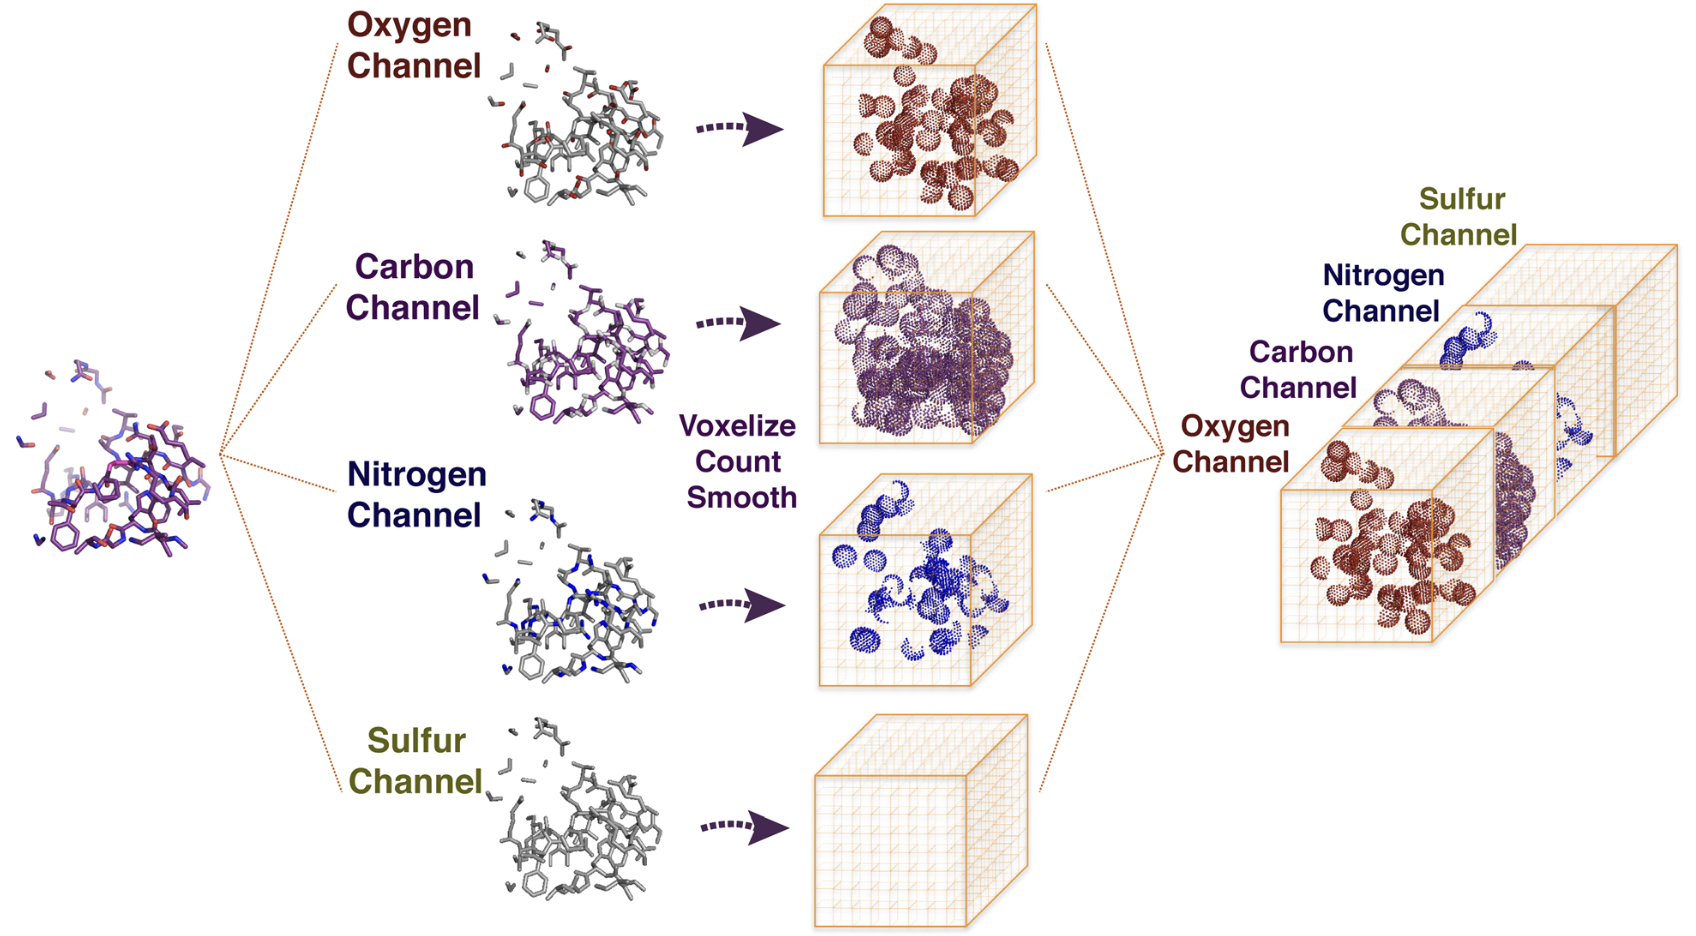
\includegraphics[width=0.7\textwidth]{masters-report/figures/3d-cnn.png}
    \caption{Local environment processing with 3D-CNNs. The local structure is first decomposed into separate atom channels. Each atom type channel is divided into 3D voxels, with each voxel recording the presence of that atom type within its boundaries. The decomposed approximation of the initial structure is then processed as it is usual with CNNs. Image taken from \cite{torng20173d}.}
    \label{3d-cnn}
\end{figure}

Based on this approach, \citet{mutcompute} introduce MutCompute, a model trained to predict the identity of an amino acid based on its local environment. \citet{mutcompute} use a different, proprietary dataset to the one used in this project. In a similar manner to the one we employ, the scores generated by the trained model are used for mutation generation across 3 proteins. More recently, \citet{Lu2022} also use MutCompute to engineer more thermally stable plastic degrading enzymes. 

In contrast to \citet{mutcompute} and \citet{Lu2022}, in this project we avoid the need of discretising the protein structure into cubic grids and therefore take full advantage of the structural properties of the atomic envrionment. To this extent, we employ equivariant graph neural networks (EGNNs), a type of GNNs that use specialised operations and architectures that preserve the structural properties of certain symmetry groups – in our case, the SE(3) group. 

\section{Equivariant graph neural networks}

Graph neural networks were proposed as a solution to dealing with graph-based data through the message-passing framework. One of the first successful architectures was the GCN, proposed by \citet{gcn}. 
Traditional GNNs operate on graphs that represent abstract collections of objects, such as social networks. To deal with geometric graphs, the message-passing paradigm was extended to include \textbf{equivariant graph neural networks} (EGNNs), a type of GNNs that can transform \textit{vector features} under some group action.

One line of research into EGNNs achieves equivariance in the E(3) and SE(3) spaces by using irreducible representations to create equivariant operations through Spherical Harmonics and Clebsch-Gordan coefficients \cite{thomas2018tensor, anderson2019cormorant, batatia2022design, fuchs2020se}. More recently, \citet{mace} use this approach to create higher-order tensor features that can more expressively model atomic environments, while \citet{liao2023equiformer} combine the Transformer architecture with the message-passing framework to include equivariant features for atom graphs. The architectures of \citet{mace} and \citet{liao2023equiformer} were both candidates for this project; however, since these approaches construct higher-order tensors, they proved to be too costly in terms of memory and training time to be applied to the large number of molecular graphs present in the ATOM3D dataset. 

The second line of research alleviates the memory cost imposed by modelling equivariant function spaces by implementing equivariant operations directly in the original Cartesian coordinates. The first model of this kind was the E$(n)$-GNN, proposed by \citet{satorras2021n}, followed by PaiNN \cite{schutt2021equivariant}. In this project, we use the GVP architecture \cite{gvp1, gvp2} and the EQGAT architecture \cite{eqgat, eqgat2}. Both implement equivariant transformations in the original Cartesian space, and have achieved state-of-the-art performance on several molecular tasks, including residue identity prediction.



